\documentclass[12pt]{article}

\usepackage[utf8]{inputenc}
\usepackage[russian]{babel}
\usepackage{amsmath}
\usepackage{setspace}

\usepackage{caption}
\usepackage{subcaption}
\usepackage{float}
\usepackage{graphicx}
\graphicspath{ {./images/} }

\usepackage{geometry}
 \geometry{
 a4paper,
 left=20mm,
 right=20mm,
 top=20mm,
 bot=20mm,
 }

\begin{document}

\begin{titlepage}
\begin{center}
    {\small НАЦИОНАЛЬНЫЙ ИССЛЕДОВАТЕЛЬСКИЙ УНИВЕРСИТЕТ ИТМО} \\
    {\small Факультет систем управления и робототехники} \\
    \vspace*{10\baselineskip}
    {\LARGEЭлектроника и схемотехника} \\
    \ \\
    \begin{spacing}{1.5}
    {\large Лабораторная работа №6 \\
    Исследование работы мультивибратора} \\
    \end{spacing} \\
    \ \\
    Вариант 2 \\
    \vspace*{10\baselineskip}
    \hfill {Выполнили студенты:} \\
    \hfill {Кирбаба Д.Д. R3338} \\
    \hfill {Курчавый В.В. R3338} \\
    \ \\
    \hfill {Преподаватель:} \\
    \hfill {Николаев Н.А.} \\
    \mbox{}
    \vfill {г. Санкт-Петербург\\2023}
\end{center}
\end{titlepage}

\section*{Цель работы}
Моделирование и исследование работы мультивибратора в LtSpice.

\section*{Ход работы}
Вариант 2.\\
Параметры:
\[
    E = 8 \ V, \ R_1 = R_4 = 3 \ kOhm,\ R_2 = R_3 = 80 kOhm, \ T = 0.5 \ sec.
\]
Рассчитаем значение емкости конденсаторов в схеме мультивибратора:
\[
    \begin{split}
        & T = 0.7(R_3C_2 + R_2C_1) \\
        & T = 0.7C(160\cdot 10^3) \\
        & C = C_1 = C_2 = \frac{T}{0.7*160\cdot 10^3} \\
        & C = 0.0044643 \cdot 10^{-3} = 4.4643 \mu F.
    \end{split}
\]
\begin{figure}[H]
    \centering
    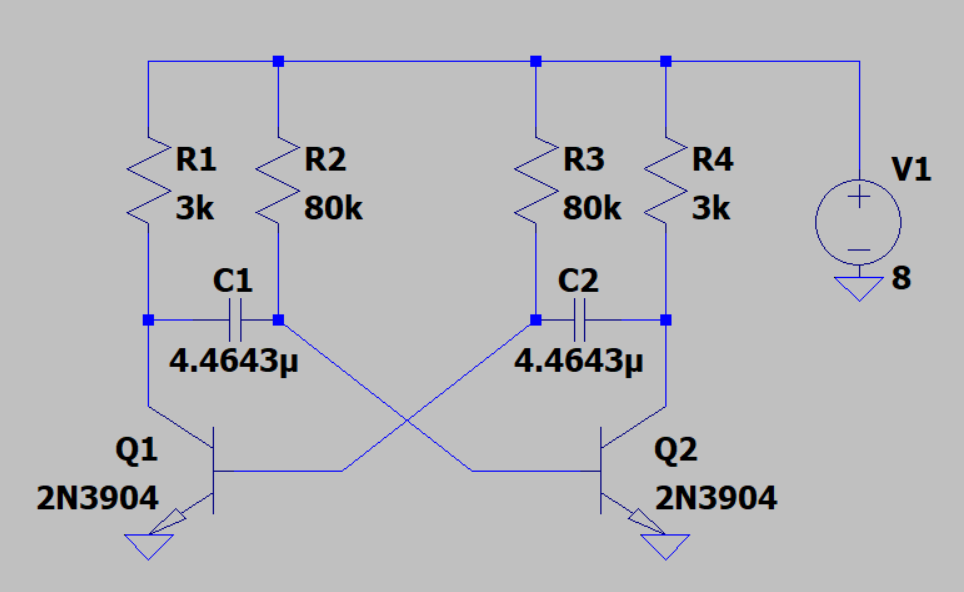
\includegraphics[width=0.7\textwidth]{scheme.png}
    \caption{Схема мультивибратора.}
    \label{fig:scheme}
\end{figure}

\begin{figure}[H]
    \centering
    \includegraphics[width=\textwidth]{plots.png}
    \caption{Графики напряжений баз и коллекторов 1 и 2 транзисторов при работе мультивибратора.}
    \label{fig:plots}
\end{figure}
На графиках можем наблюдать два состояния мультивибратора: когда один из транзисторов находится в режиме насыщения, другой - в режиме отсечки и наоборот. \\
\ \\
Определим период сгенерированного сигнала:
\[
    \begin{split}
        T = 0.7(R_3C_2 + R_2C_1) = 1.4R_2C_1 = 0.5 \ sec.
    \end{split}
\]
Рассчитаем скважность:
\[
    Q = \frac{T}{t_{int}} = \frac{0.5}{0.25} = 2.
\]
Скважность - отношение периода повторения к длительности импульса.

\section*{Выводы}
Объектом исследования данной работы были мультивибраторы. Это приборы для колебаний почти прямоугольных сигналов. \\
Мультивибратор может работать в автоколебательном режиме, режиме синхронизации и ждущем режиме. \\
\ \\
В этой работе исследовался автоколебательный режим мультивибратора. Была построена схема моделирования, а затем переходные процессы при подаче напряжения. \\
На графиках можно было наглядно увидеть переодические смены квазисостояний.\\
В конце были рассчитаны период и скважность системы.

\end{document}